\documentclass{standalone}
\usepackage{tikz}
\usepackage{ctex,siunitx,ninecolors}
\usepackage{tkz-euclide}
\usepackage{amsmath}
\usetikzlibrary{patterns, calc}
\usetikzlibrary {decorations.pathmorphing, decorations.pathreplacing, decorations.shapes,}
\begin{document}
\small
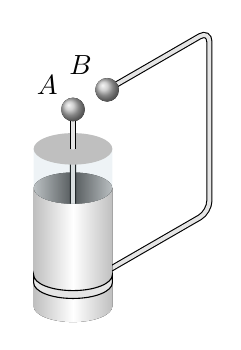
\begin{tikzpicture}[>=stealth]
  \fill[left color=lightgray,right color=lightgray,middle color=darkgray](0,-1.0)ellipse(0.5 and 0.2);
  \draw[double=lightgray!40,rounded corners,double distance=0.5mm](30:0.5)--(30:2.0)--++(0,-2.3)--++(-150:2.0)--++(0,1.9);
  \fill[ball color=lightgray](30:0.5)circle(0.15)node[above left=1mm]{$B$};
  \fill[left color=lightgray,right color=lightgray,middle color=white]
  (-0.5,-1.0)--(-0.5,-2.5)arc(-180:0:0.5 and 0.2)--(0.5,-1.0)arc(0:-180:0.5 and 0.2);
  \fill[cyan!20!lightgray,opacity=0.2](-0.5,-1.0)arc(-180:0:0.5 and 0.2)--(0.5,-0.5)--(-0.5,-0.5)--cycle;
  \fill[lightgray](0,-0.5)ellipse(0.5 and 0.2);
  \fill[lightgray!40](0,-0.5)ellipse(0.025 and 0.01);
  \draw[double=lightgray!40,double distance=0.5mm](0,-0.5)--(0,0);
  \fill[ball color=lightgray](0,0)circle(0.15)node[above left=1mm]{$A$};
  \draw[fill=lightgray!40](-0.5,-2.2)arc(-180:0:0.5 and 0.2)--(0.5,-2.1)arc(0:-180:0.5 and 0.2)--cycle;
\end{tikzpicture}
\end{document}